\documentclass[12pt,a4paper]{scrartcl}
\usepackage{listings}
\usepackage[utf8]{inputenc}
\usepackage{mathtools}
\usepackage[english,russian]{babel}
\usepackage{indentfirst}
\usepackage{misccorr}
\usepackage{graphicx}
\usepackage{amsmath}
\usepackage[rightcaption]{sidecap}
\usepackage{wrapfig}
\usepackage{mathptmx}
\usepackage{graphicx}
\usepackage{multicol}

\begin{document}

\begin{titlepage}
  \begin{center}
     
    \vspace{0.5cm}
 
    НОВОСИБИРСКИЙ ГОСУДАРСТВЕННЫЙ УНИВЕРСИТЕТ
    \vspace{0.25cm}
     
    Механико-математический факультет
     
    Кафедра: Математика и компьютерные науки
    \vfill
     
     
    Тлепбергенова Дарья Дулатовна
    \vfill
 
    \textsc{Отчет по предмету: Графы и алгоритмы}\\[5mm]
     
    {\LARGE Алгоритм Дейкстры. \\
    Поиск минимального пути в графе.\\[2mm]}
  \bigskip
     
    3 курс, группа 16121
\end{center}
\vfill
 \newlength{\ML}
\settowidth{\ML}{«\underline{\hspace{0.7cm}}» \underline{\hspace{2cm}}}
\hfill\begin{minipage}{0.4\textwidth}
  Преподаватель:\\
  Хомякова Екатерина Николаевна
\end{minipage}%
\bigskip

 \vfill
\begin{center}
  Новосибирск, 2018 г.
\end{center}
\end{titlepage}

\newpage
\section{Постановка задачи.}

Для заданного графа (в том числе и несвязного) $G=(V,E)$ найти все блоки графа.

\section{Описание алгоритма.}

Запустим обход в глубину из произвольной вершины графа,обозначим ее через root (корень). Заметим следующий факт (который несложно доказать):

Пусть мы находимся в обходе в глубину, просматривая сейчас все рёбра из вершины $u \neq root$. Тогда, если текущее ребро $(u,v)$ таково, что из вершины $v$ и из любого её потомка в дереве обхода в глубину нет обратного ребра в какого-либо предка вершины $u$, то вершина $u$ является точкой сочленения. В противном случае, т.е. если обход в глубину просмотрел все рёбра из вершины v, и не нашёл удовлетворяющего вышеописанным условиям ребра, то вершина $u$ не является точкой сочленения. (В самом деле, мы этим условием проверяем, нет ли другого пути из $u$ в $v$)

Рассмотрим теперь оставшийся случай: $v = root$. Тогда эта вершина является точкой сочленения тогда и только тогда, когда эта вершина имеет более одного сына в дереве обхода в глубину. (В самом деле, это означает, что, пройдя из $root$ по произвольному ребру, мы не смогли обойти весь граф, откуда сразу следует, что $root$ — точка сочленения).

Теперь осталось научиться проверять этот факт для каждой вершины эффективно. Для этого воспользуемся "временами входа в вершину", вычисляемыми алгоритмом поиска в глубину.

Итак, пусть $visitedVertex[v]$ — это время захода поиска в глубину в вершину u. Теперь введём массив $low[v]$, который и позволит нам отвечать на вышеописанные запросы. Время $low[v]$ равно минимуму из времени захода в саму вершину $visitedVertex[v]$, времён захода в каждую вершину $v$, являющуюся концом некоторого обратного ребра $(u,v)$, а также из всех значений $low[v]$ для каждой вершины $v$, являющейся непосредственным сыном $u$ в дереве поиска:

\[
 low[u] = \min \begin{cases}
                    visitedVertex[u],\\
                    visitedVertex[v]\text{  } \forall (u,v) - \text{обратное ребро}\\
                    low[v]\text{  }  \forall (u,v) - \text{ребро дерева}
                    \end{cases}
\]

Тогда, из вершины $u$ или её потомка есть обратное ребро в её предка тогда и только тогда, когда найдётся такой сын $v$, что $low[v] < visitedVertex[u]$.

Таким образом, если для текущего ребра $(u,v)$ (принадлежащего дереву поиска) выполняется $low[v] \le visitedVertex[u]$, то вершина $u$ является точкой сочленения. Для начальной вершины $u = root$ критерий другой: для этой вершины надо посчитать число непосредственных сыновей в дереве обхода в глубину.

\section{Код программы.}

\subsection{Класс Graph}
	\begin{verbatim}
	/*
 * Задание: Для зананного графа найти все его блкои и выдать их.
 */

import java.util.*;

class Graph {
    private int vertexCount; // - количество связей
    private LinkedList[] adj; // - лист связей

    /**
     * time - ипользуется как глобальная переменная для отслеживания
     * нумирации прохождения вершин (какая попала 1й.2й ...).
     * biconnectedComponentsCount - количество компонент
     двусвязности(блоков) графа.
     */

    int biconnectedComponentsCount = 0;
    private int time = 0;

    /**
     * Класс ребер, из которых будет состоять Граф
     */
    private class Edge {
        int u;
        int v;

        Edge(int u, int v) {
            this.u = u;
            this.v = v;
        }
    }

    /**
     * Данный конструктор создает пустой граф
     *
     * @param vertexCount - количество вершин в создоваемом графе
     */
    Graph(int vertexCount) {
        this.vertexCount = vertexCount;
        adj = new LinkedList[vertexCount];
        for (int i = 0; i < vertexCount; ++i)
            adj[i] = new LinkedList();
    }

    /**
     * функция добавления направленного ребра в граф
     *
     * @param vertexInput  - вершина, из которой выходит ребро
     * @param vertexOutput - вершина, в которую входит ребро
     */
    void addEdge(int vertexInput, int vertexOutput) {
        adj[vertexInput].add(vertexOutput);
    }

    /**
     * Конструктор графа по матрице смежности
     *
     * @param matrix - матрица смежности
     */
    Graph(double[][] matrix) {
        vertexCount = matrix.length;
        adj = new LinkedList[matrix.length];
        for (int i = 0; i < matrix.length; ++i) {
            adj[i] = new LinkedList();
            for (int j = 0; j < matrix.length; ++j) {
                if (matrix[i][j] != 0) {
                    adj[i].add(j);
                }
            }
        }
    }

    /**
     * Рекурсивная функция, которая находит и печатает
     * компоненты связности, использующие обход DFS
     *
     * @param u             - посещаемая вершина
     * @param visitedVertex - массив для отслеживания
     * посещенных вершин по времени
     * @param low           - самая первая вершина (вершина с
     * минимальным временем обнаружения),
     *                      которая может быть достигнута из
     * поддерева
     * @param st            - стек, поддерево в глубину.
     * @param parent        - "родители вершины"
     */
    private void DFSForBlocks(int u, int visitedVertex[], int
    low[], LinkedList<Edge> st,
                              int parent[]) {
        //отмечаем, что поситили вершину и запомнили какой по
        //счету пришла
        visitedVertex[u] = low[u] = ++time;
        //изначально детей у нее нет
        int children = 0;

        // проходим по всем вершинам, с которыми соеденина эта
        // вершина ребрами
        Iterator<Integer> it = adj[u].iterator();
        while (it.hasNext()) {
            // v - вершина, смежная с u
            int v = it.next();

            // если мы ее (v) еще не посещали
            if (visitedVertex[v] == -1) {
                children++;
                parent[v] = u;

                // заносим в стек
                st.add(new Edge(u, v));
                // запускаем рекурсивно уже от v
                DFSForBlocks(v, visitedVertex, low, st, parent);


                //проверяем связанно ли поддерево из v с
                //предками u (проверка определения точки
                //сочлинения)
                if (low[u] > low[v]) {
                    low[u] = low[v];
                }

                //если u - точка сочлинения выводим все ребра
                //из стека до ребра u-v
                if ((visitedVertex[u] == 1 && children > 1) ||
                (visitedVertex[u] > 1 && low[v] >= visitedVertex[u])) {
                    while (st.getLast().u != u || st.getLast().v != v) {
                        System.out.print(st.getLast().u + "-" +
                        st.getLast().v + " ");
                        st.removeLast();
                    }
                    System.out.println(st.getLast().u + "-" +
                    st.getLast().v + " ");
                    st.removeLast();

                    biconnectedComponentsCount++;
                }
            }

            // изменяем значение low[u] если нашли более быстрый
            else if (v != parent[u] && visitedVertex[v] < low[u]) {
                if (low[u] > visitedVertex[v])
                    low[u] = visitedVertex[v];
                st.add(new Edge(u, v));
            }
        }
    }

    /**
     * Функция для обхода DFS.
     */
    void findBlocks() {
        int visitedVertex[] = new int[vertexCount];
        int low[] = new int[vertexCount];
        int parent[] = new int[vertexCount];
        LinkedList<Edge> st = new LinkedList<Edge>();

        // автозаполнение массивов -1-ми
        Arrays.fill(visitedVertex, -1);
        Arrays.fill(low, -1);
        Arrays.fill(parent, -1);

        for (int i = 0; i < vertexCount; i++) {
            //для каждой непосещенной вершины:
            if (visitedVertex[i] == -1)
                DFSForBlocks(i, visitedVertex, low, st, parent);

            boolean incBiconnectedComponent = false;

            // если стек не пустой, то печатаем его ребра
            while (st.size() > 0) {
                incBiconnectedComponent = true;
                System.out.print(st.getLast().u + "-" + st.getLast().v + " ");
                st.removeLast();
            }
            if (incBiconnectedComponent) {
                System.out.println();
                biconnectedComponentsCount++;
            }
        }
    }
}
	\end{verbatim}
	\subsection{Класс Main}
	\begin{verbatim}
	    public class Main {
    /**
     * Main - функция с примерами
     */
    public static void main(String[] args) {
        //Пример 1
        Graph graph1 = new Graph(new double[][]{
                {0, 1, 0, 0, 0, 0, 1, 0, 0, 0, 0, 0},
                {1, 0, 1, 1, 0, 1, 0, 0, 0, 0, 0, 0},
                {0, 1, 0, 1, 1, 0, 0, 0, 0, 0, 0, 0},
                {0, 1, 1, 0, 1, 0, 0, 0, 0, 0, 0, 0},
                {0, 0, 1, 1, 0, 0, 0, 0, 0, 0, 0, 0},
                {0, 1, 0, 0, 0, 0, 1, 1, 1, 0, 0, 0},
                {1, 0, 0, 0, 0, 1, 0, 0, 0, 0, 0, 0},
                {0, 0, 0, 0, 0, 1, 0, 0, 1, 0, 0, 0},
                {0, 0, 0, 0, 0, 1, 0, 1, 0, 1, 0, 0},
                {0, 0, 0, 0, 0, 0, 0, 0, 1, 0, 0, 0},
                {0, 0, 0, 0, 0, 0, 0, 0, 0, 0, 0, 1},
                {0, 0, 0, 0, 0, 0, 0, 0, 0, 0, 1, 0}
        });
        System.out.println("Пример 1:");
        graph1.findBlocks();
        System.out.println("Количество блоков = " +
        graph1.biconnectedComponentsCount);

        //Пример 2
        Graph graph2 = new Graph(7);
        System.out.println("Пример 2:");
        graph2.addEdge(0, 1);
        graph2.addEdge(1, 3);
        graph2.addEdge(0, 3);
        graph2.addEdge(3, 4);
        graph2.addEdge(1, 4);
        graph2.addEdge(2, 4);
        graph2.addEdge(4, 5);
        graph2.addEdge(2, 5);
        graph2.addEdge(5, 6);
        graph2.addEdge(1, 0);
        graph2.addEdge(3, 1);
        graph2.addEdge(3, 0);
        graph2.addEdge(4, 3);
        graph2.addEdge(4, 1);
        graph2.addEdge(4, 2);
        graph2.addEdge(5, 4);
        graph2.addEdge(5, 2);
        graph2.addEdge(6, 5);
        graph2.findBlocks();
        System.out.println("Количество блоков = " +
        graph2.biconnectedComponentsCount);
    }
}
	\end{verbatim}

	\newpage
\section{Тесты.}

\subsection{Пример 1:}
	\begin{figure}[h]
	\begin{multicols}{2}
		\hfill
		\includegraphics[width=70mm]{BiconnectedComponent.png}
		\hfill
		\caption{Грраф из Примера 1}
		\hfill
		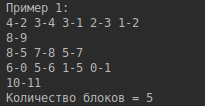
\includegraphics[width=70mm]{ex1.png}
		\hfill
		\caption{Результат программы}
	\end{multicols}
\end{figure}

\begin{figure}[h]
	\begin{multicols}{2}
		\hfill
		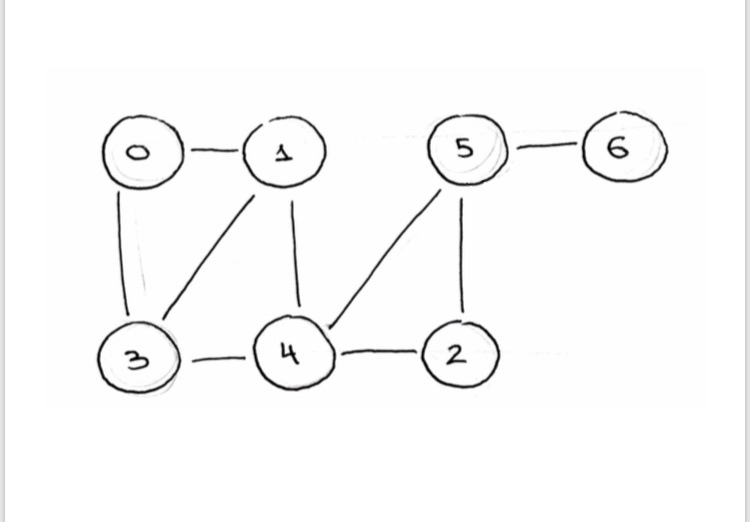
\includegraphics[width=50mm]{graph2.jpg}
		\hfill
		\caption{Граф из Примера 2}
		\hfill
		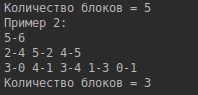
\includegraphics[width=70mm]{ex2.png}
		\hfill
		\caption{Результат программы}
	\end{multicols}
\end{figure}

\section{Выводы.}

 Двусвязность графа - очень желательный признак для некоторых приложений. Представим себе, что вершины графа изображают узлы некоторой информационной сети, а ребра соответствуют линиям передачи. Если наш граф двусвязный, то выход из строя отдельного узла w никогда не приведет к потере соединения между любыми двумя узлами, отличными от w. Знание блоков графа также очень важно, если принять во внимание то, что многие графовые задачи, такие как нахождение всех элементарных циклов или установление факта планарности графа (граф называется планарным, если его можно так начертить на плоскости, чтобы никакие два ребра не пересекались), приводят естественным путем к аналогичным задачам для блоков данного графа.
\end{document}
